\documentclass[presentation]{beamer}
\usepackage[utf8]{inputenc}
\usepackage[T1]{fontenc}

% \usepackage{etex}


% \usepackage{tikz}

% \usepackage{amsfonts}
% \usepackage{tikz}
% \usepackage{caption}
% \usepackage{subcaption}

\usepackage[inline]{asymptote}
\usepackage{attachfile2}
\usepackage{asyfig}


\definecolor{links}{HTML}{2A1B81}
\hypersetup{colorlinks,linkcolor=,urlcolor=magenta}
\useinnertheme[shadow,outline]{chamfered}
\usecolortheme{beaver}
\beamertemplatenavigationsymbolsempty
\usefonttheme{professionalfonts}

\let\digamma\relax
\usepackage[scale=0.85,stdmathitalics=true,romanfamily=casual]{lucimatx}

\usepackage[scaled=0.85]{zi4}  % inconsolata font
\renewcommand*\familydefault{\ttdefault}

\usefonttheme[stillsansseriftext]{serif}






%===========================================================
% Title Info
\title{Logistic Regression}

\author{Instructor: Paul M. Magwene}


\begin{document}
%===========================================================
\begin{frame}
\titlepage
\end{frame}




%===========================================================
\begin{frame}
  \frametitle{Logistic Regression}
  
Logistic regression is used when the dependent variable is discrete (often binary).  The explanatory variables may be either continuous or discrete.
\medskip

Examples:
\begin{itemize}
\item whether a gene is turned off (=0) or on (=1) as a function of levels of various proteins
\item whether an individual is healthy (=0) or diseased (=1) as a function of various risk factors.
\item whether an individual animal died (=0) or survived (=1) some selective event as a function of one or more moprhological traits.
\end{itemize}


\end{frame}

%===========================================================
\begin{frame}
  \frametitle{Logistic Regression}

Model the binary responses as:

\[P(Y = 1|X_1,\ldots,X_p) = f(\beta_0 + \beta_1 x_1 + \beta_2 x_2 + \cdots + \beta_p x_p)
\]

So we're modeling the probability of the states as a function of a linear combination of the predictor variables.

\medskip


For logistic regression, $f$ is thus the logistic function:

\[
f(z) = \frac{e^z}{1+e^z} = \frac{1}{1 + e^{-z}}
\]

\end{frame}

%===========================================================
\begin{frame}
  \frametitle{Binary Logistic Regression}

$Y$ is a binary response variable (0, 1)

$X$ is a continuous predictor variable 

\[
P(Y = 1 | X) = \frac{1}{1+e^{-(\beta_0 + \beta_1 X)}}
\]

\bigskip

\begin{center}
\asyinclude[height=1.25in,keepAspect=true]{logistic-fxn.asy}
\end{center}

\end{frame}

%===========================================================
\begin{frame}
  \frametitle{Notes on Logistic Regression}

\begin{itemize}
    \item The regression is no longer linear
    \item Estimating the $\beta$ in logistic regression is done via maximum likelihood estimation (MLE)
\end{itemize}

\end{frame}

%===========================================================
\begin{frame}
  \frametitle{Logistic Regression Example: Sinking of the Titanic}
  
\begin{figure}
\begin{center}
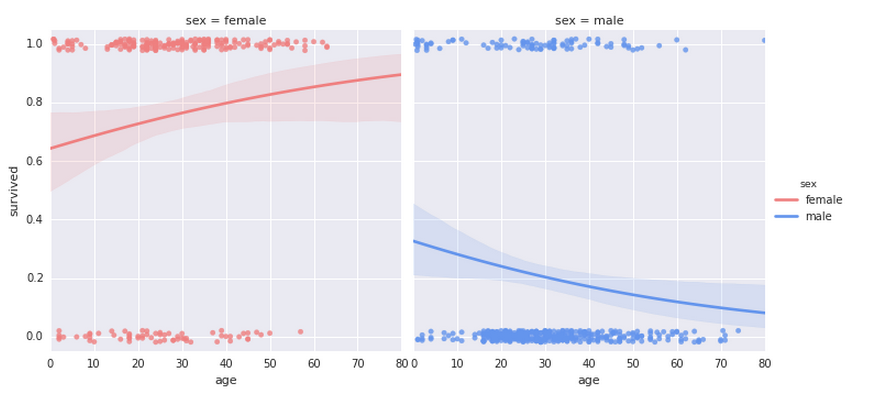
\includegraphics[height=2in]{titanic_survival.png}
\end{center}
\end{figure}




\end{frame}
%===========================================================




\end{document}


%===========================================================
\begin{frame}
  \frametitle{XXX}

\end{frame}
%===========================================================
